\documentclass[xcolor=svgnames,professionalfonts,11pt,aspectratio=43,handout]{beamer}

%!TEX root = ../thesis.tex

\usepackage[utf8]{inputenc}
\usepackage[T1]{fontenc}
\usepackage[english]{babel}

\usepackage{etoolbox}
\pretocmd{\section}{\clearpage}{}{}

\usepackage{amssymb}

\usepackage{libertine}
\usepackage[scaled=0.83]{beramono}
\usepackage{textcomp}
\usepackage{setspace}
\setlength{\parindent}{0em}
\usepackage[svgnames]{xcolor}
\usepackage{graphicx}
\usepackage{tabularx}

\newcolumntype{b}{>{\bfseries}c}

\usepackage{booktabs}
\usepackage{multirow}

\usepackage{multicol}
\usepackage{lipsum}

\usepackage{listings}
%!TEX root = ../thesis.tex
\definecolor{comment}{HTML}{236E25}
\definecolor{keyword}{HTML}{881280}
\definecolor{ndkeyword}{HTML}{994500}
\definecolor{string}{HTML}{1A1AA6}

\makeatletter
\newcommand{\miniscule}{\@setfontsize\miniscule{5}{6}}% \tiny: 6/7
\makeatother

\lstset{%
  basicstyle=\ttfamily\scriptsize\mdseries\singlespacing,
  %columns=fullflexible,
  breakatwhitespace=false,
  breaklines=true,
  numbers=left,
  numberstyle=\ttfamily\scriptsize,
  stepnumber=5,
  numberfirstline=false,
  firstnumber=1,
  showstringspaces=false,
  tabsize=2,
  backgroundcolor=\color{white},
  captionpos=t,
  frame=L,
  float=htb,
  xleftmargin=\bigskipamount,
  xrightmargin=\bigskipamount,
  aboveskip=\bigskipamount,
  belowskip=\bigskipamount,
  commentstyle=\color{comment},
  stringstyle=\color{string},
  identifierstyle=\color{black},
  keywordstyle=\color{keyword}\bfseries,
  ndkeywordstyle=\color{ndkeyword},
}

\lstset{literate=
  {á}{{\'a}}1 {é}{{\'e}}1 {í}{{\'i}}1 {ó}{{\'o}}1 {ú}{{\'u}}1
  {Á}{{\'A}}1 {É}{{\'E}}1 {Í}{{\'I}}1 {Ó}{{\'O}}1 {Ú}{{\'U}}1
  {à}{{\`a}}1 {è}{{\'e}}1 {ì}{{\`i}}1 {ò}{{\`o}}1 {ù}{{\`u}}1
  {À}{{\`A}}1 {È}{{\'E}}1 {Ì}{{\`I}}1 {Ò}{{\`O}}1 {Ù}{{\`U}}1
  {ä}{{\"a}}1 {ë}{{\"e}}1 {ï}{{\"i}}1 {ö}{{\"o}}1 {ü}{{\"u}}1
  {Ä}{{\"A}}1 {Ë}{{\"E}}1 {Ï}{{\"I}}1 {Ö}{{\"O}}1 {Ü}{{\"U}}1
  {â}{{\^a}}1 {ê}{{\^e}}1 {î}{{\^i}}1 {ô}{{\^o}}1 {û}{{\^u}}1
  {Â}{{\^A}}1 {Ê}{{\^E}}1 {Î}{{\^I}}1 {Ô}{{\^O}}1 {Û}{{\^U}}1
  {œ}{{\oe}}1 {Œ}{{\OE}}1 {æ}{{\ae}}1 {Æ}{{\AE}}1 {ß}{{\ss}}1
  {ç}{{\c c}}1 {Ç}{{\c C}}1 {ø}{{\o}}1 {å}{{\r a}}1 {Å}{{\r A}}1
  {€}{{\EUR}}1 {£}{{\pounds}}1 {°}{{\textdegree}}1
  {µ}{{$\mathrm{\mu}$}}1
  {±}{{$\pm$}}1
  {σ}{{$\mathrm{\sigma}$}}1
  {⋅}{{$\cdot$}}1
}
\lstdefinelanguage{JavaScript}{
  morekeywords={break, case, catch, continue, debugger, default, delete, do, else, finally, for, function, if, in, instanceof, new, return, switch, this, throw, try, typeof, var, while, with, null, throw, this},
  morendkeywords={Object,Array,Boolean,Date,window,Number,String,Math,XMLHttpRequest,document,prototype,undefined,Infinity,NaN,import,export,this,console,Error},
  sensitive,
  comment=[l]{//},
  morecomment=[s]{/*}{*/},
  morestring=[b]',
  morestring=[b]",
}
\lstdefinelanguage{XML}{
  morestring=[b]",
  morecomment=[s]{<?}{?>},
  morecomment=[s]{<!--}{-->},
  morecomment=[s]{&}{;},
  alsoletter={:},
  morekeywords={
    ComplexData,
    ComplexOutput,
    DataInputs,
    Default,
    Encoding,
    Format,
    hello,% remove,
    Input,
    LiteralData,
    LiteralOutput,
    MimeType,
    Output,
    ows:Abstract,
    ows:AnyValue,
    ows:DataType,
    ows:Identifier,
    ows:LowerCorner,
    ows:Title,
    ows:UOM,
    UOMs,
    ows:UpperCorner,
    ProcessDescription,
    ProcessOutputs,
    soap:Body,
    soap:Envelope,
    soap:Header,
    stream:InputMessage,
    stream:Inputs,
    stream:Output,
    stream:OutputMessage,
    stream:OutputRequestMessage,
    stream:Outputs,
    stream:ProcessID,
    ows:AllowedValues,
    ows:Value,
    stream:Reference,
    stream:ReferenceInput,
    stream:StopMessage,
    stream:StreamingInput,
    Supported,
    wps:BoundingBoxData,
    wps:ComplexData,
    wps:Data,
    wps:DataInputs,
    wps:Execute,
    wps:ExecuteResponse,
    wps:Input,
    wps:LiteralData,
    wps:Output,
    wps:Process,
    wps:ProcessDescriptions,
    wps:ProcessOutputs,
    wps:ProcessSucceeded,
    wps:Reference,
    wps:Status,
    wsa:Action,
    wsa:Address,
    wsa:FaultTo,
    wsa:From,
    wsa:MessageID,
    wsa:RelatesTo,
    wsa:ReplyTo,
    wsa:To,
  },
  morendkeywords={
    creationTime,
    crs,
    dataType,
    dimensions,
    encoding,
    includeInputs,
    maxOccurs,
    method,
    mimeType,
    minOccurs,
    ows:reference,
    RelationshipType,
    service,
    serviceInstance,
    statusSupported,
    storeSupported,
    version,
    wps:processVersion,
    xlink:href,
    xml:lang,
    xmlns:ows,
    xmlns:soap,
    xmlns:stream,
    xmlns:wps,
    xmlns:wsa,
    xmlns:xlink,
  }
}
\newcommand{\texttag}[2]{\texttt{\tiny{\textless\textcolor{keyword}{#1:#2}\textgreater}}}
\newcommand{\includecode}[2][xml]{\lstinputlisting[]}

\usepackage{enumitem}
\setlist{nolistsep}

\usepackage[hyphens]{url}
\urlstyle{same}
\renewcommand{\UrlBreaks}{%
\do\a\do\b\do\c\do\d\do\e\do\f%
\do\g\do\h\do\i\do\j\do\k\do\l%
\do\m\do\n\do\o\do\p\do\q\do\r%
\do\u\do\v\do\w\do\x\do\y\do\z%
\do\A\do\B\do\C\do\D\do\E\do\F%
\do\G\do\H\do\I\do\J\do\K\do\L%
\do\M\do\N\do\O\do\P\do\Q\do\R%
\do\U\do\V\do\W\do\X\do\Y\do\Z%
\do\_\do\/\do\-}

%\usepackage{titlesec}
%\titleformat{\paragraph}[hang]{\sffamily\bfseries}{\theparagraph}{.5em}{}
%\titleformat{\subparagraph}[hang]{\sffamily\bfseries}{\thesubparagraph}{.5em}{}

\usepackage[unicode,breaklinks,hidelinks,colorlinks=true,urlcolor=black,linkcolor=black,citecolor=black]{hyperref}

\usepackage[authoryear,round,comma,sort&compress]{natbib}

\usepackage[margin=10pt,labelfont={bf},format=plain]{caption}

\bibliographystyle{plainnat}

\usepackage{acronym}
%!TEX root = ../thesis.tex

\acrodef{WPS}{Web Processing Service}
\acrodef{OGC}{Open Geospatial Consortium}
\acrodef{DAG}{Directed Acyclic Graph}
\acrodef{BFS}{Breadth-first search}

\usepackage{listings}

\hypersetup{
    pdftitle={Streaming Web-Services for Calculating Live Hydrological Derivatives},
    pdfsubject={Master Thesis},
    pdfauthor={Christian Autermann}
}

\newcommand{\fu}[1]{\footnote{\url{#1}}}
\newcommand{\mail}[1]{\href{mailto:#1}{#1}}



\newsavebox\mybox
\newenvironment{signedquote}[1]
  {\savebox\mybox{\small\textup{--- #1}}\begin{quote}\itshape}
  {{\leavevmode\unskip\nobreak\hfil\penalty50\hskip2em
  	\hbox{}\nobreak\hfil\usebox\mybox\parfillskip=0pt
    \finalhyphendemerits=0\endgraf}\end{quote}}

\title{Streaming Web-Services for Calculating Live Hydrological Derivatives}
\subtitle{Master Thesis Defense}
\institute{Supervisors: Edzer Pebesma (IfGI), Jordan Read (USGS CIDA)}
\author{Christian Autermann}
\date{January 31, 2014}

\begin{document}

\frame{\titlepage}

\begin{frame}[t]{Outline}
  \begin{enumerate}
    \item Introduction
    \item Lake Analyzer
    \item Matlab WPS
    \item Lake Analyzer WPS
    \item Streaming WPS
    \item Current Status
  \end{enumerate}
\end{frame}

\titleframe{Introduction}

\begin{frame}[t]{Introduction}
  \begin{itemize}
    \item
  \end{itemize}
\end{frame}

\titleframe{Lake Analyzer}

\begin{frame}[t]{Lake Analyzer}
  \begin{itemize}
    \item
  \end{itemize}
\end{frame}

\begin{frame}{Lake Analyzer --- Outputs}
  \begin{columns}
    \column{.45\textwidth}
    \begin{itemize}
      \item Raw Results
      \item Buoyancy frequency
      \item Parent buoyancy frequency
      \item Lake number
      \item Parent lake number
      \item Metalimnion bottom depth
      \item Parent metalimnion bottom depth
      \item Metalimnion top depth
      \item Parent metalimnion top depth
      \item Mode one vertical seiche period
    \end{itemize}
    \column{.45\textwidth}
    \begin{itemize}
      \item Parent mode one vertical seiche period
      \item Schmidt stability
      \item Thermocline depth
      \item Parent thermocline depth
      \item u star (turblent velocity scale from wind)
      \item Parent u star (turblent velocity scale from wind)
      \item Water temperature
      \item Wedderburn number
      \item Parent Wedderburn number
      \item Wind speed
    \end{itemize}
  \end{columns}
\end{frame}

\begin{frame}[c,fragile]{Lake Analyzer --- Outputs}
  \begin{figure}
    \centering
    \subfigure{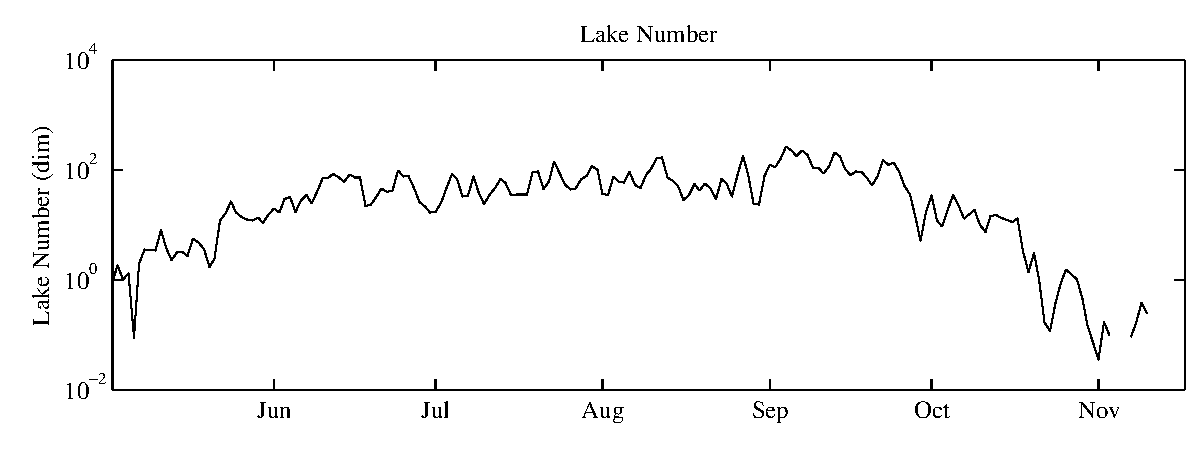
\includegraphics[width=.25\textwidth]{figures/Sparkling_Ln.pdf}}
    \subfigure{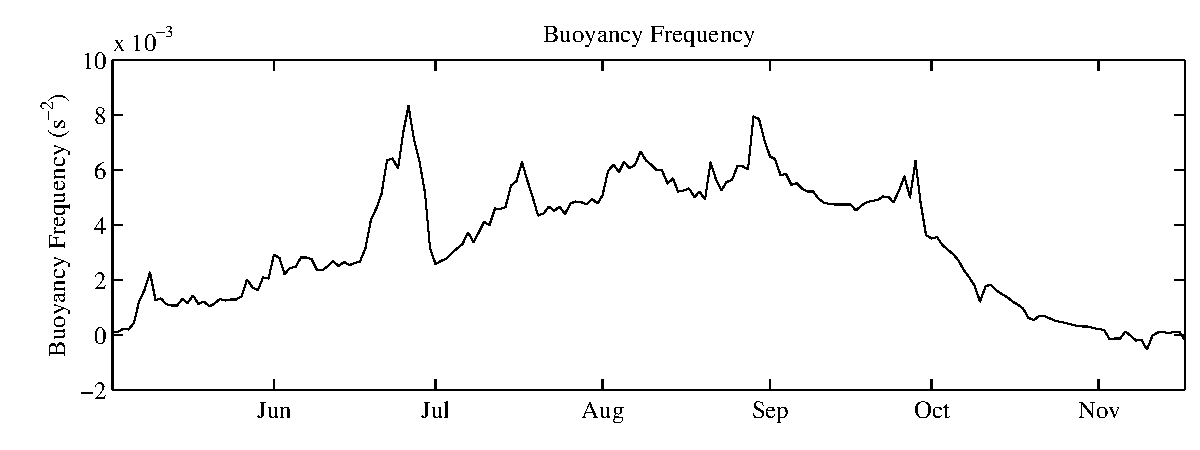
\includegraphics[width=.25\textwidth]{figures/Sparkling_N2.pdf}}
    \subfigure{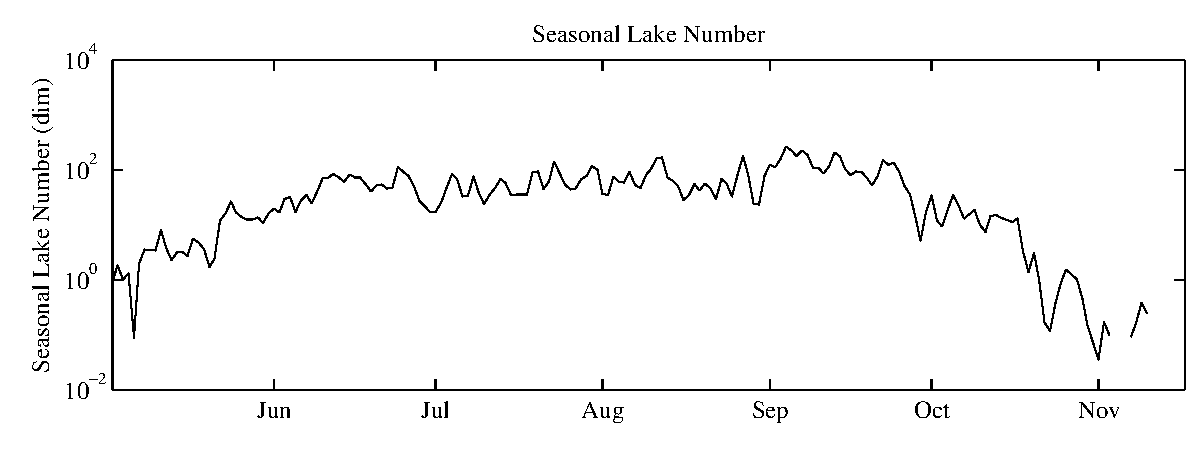
\includegraphics[width=.25\textwidth]{figures/Sparkling_SLn.pdf}}\\
    \subfigure{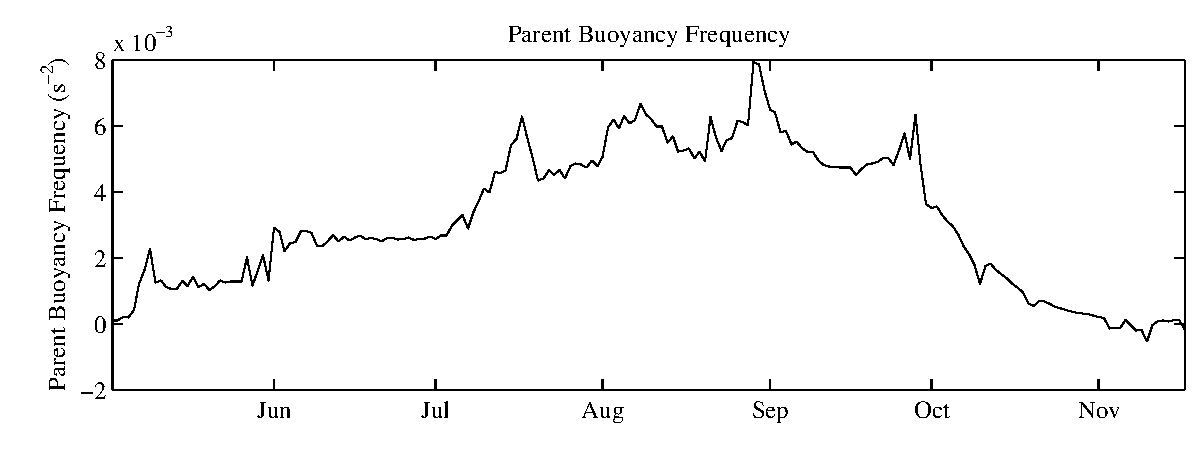
\includegraphics[width=.25\textwidth]{figures/Sparkling_SN2.pdf}}
    \subfigure{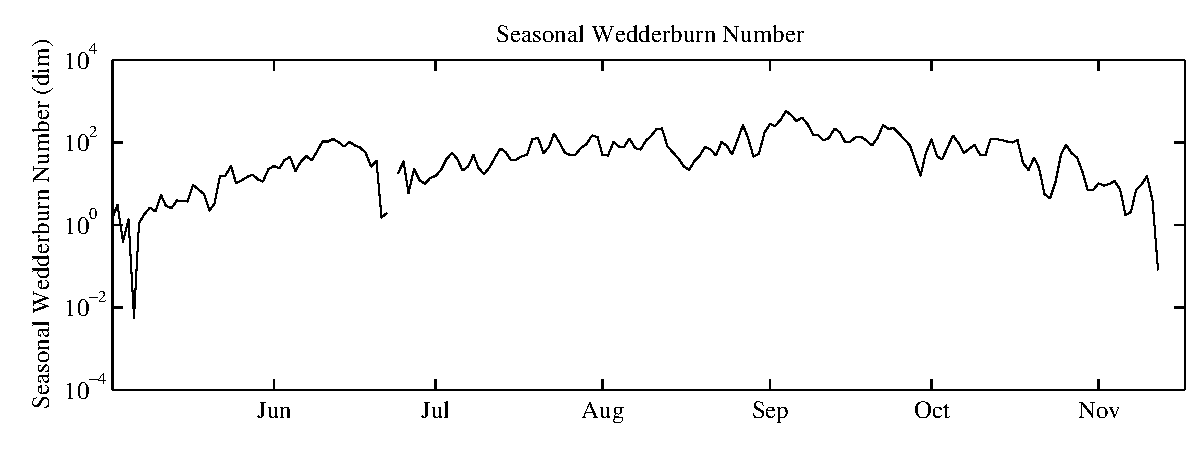
\includegraphics[width=.25\textwidth]{figures/Sparkling_SW.pdf}}
    \subfigure{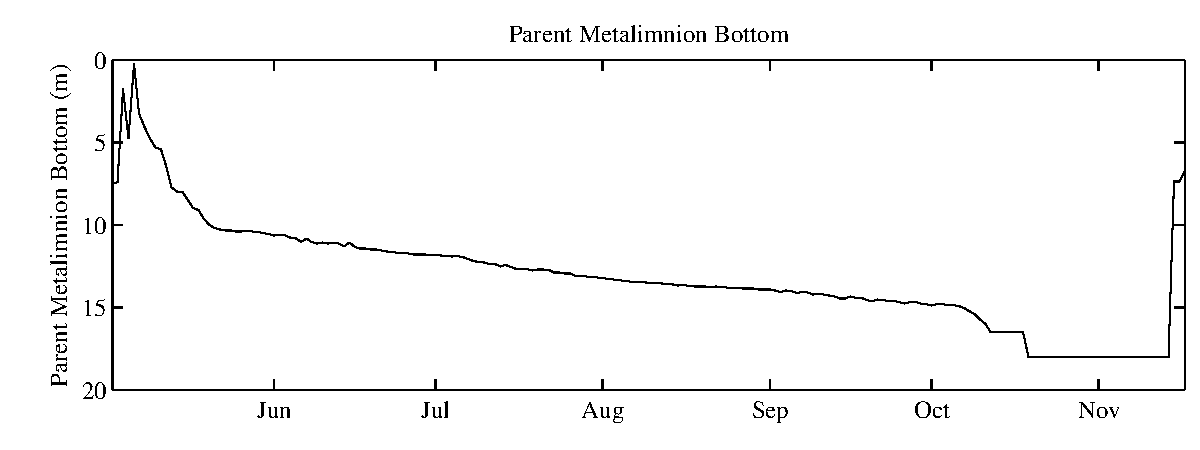
\includegraphics[width=.25\textwidth]{figures/Sparkling_SmetaB.pdf}}\\
    \subfigure{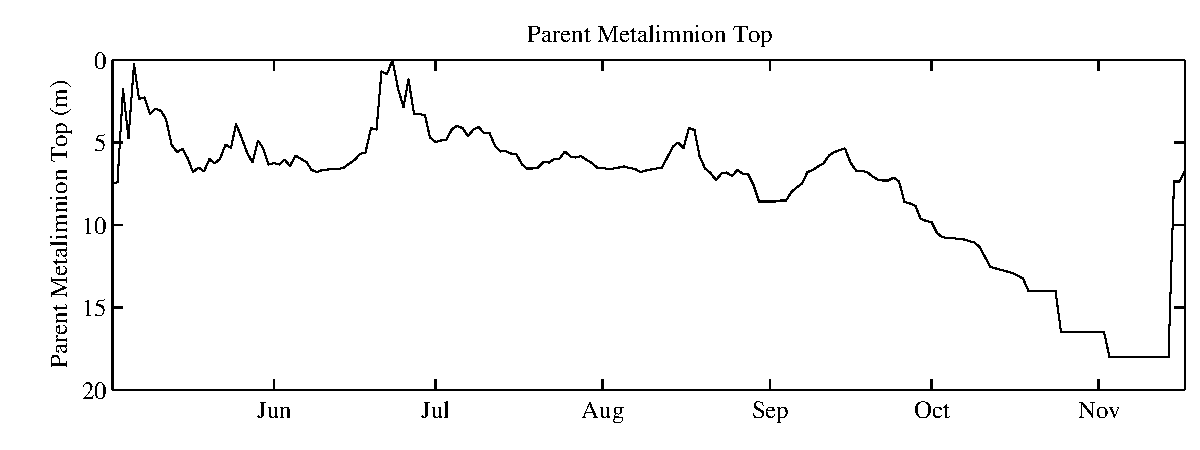
\includegraphics[width=.25\textwidth]{figures/Sparkling_SmetaT.pdf}}
    \subfigure{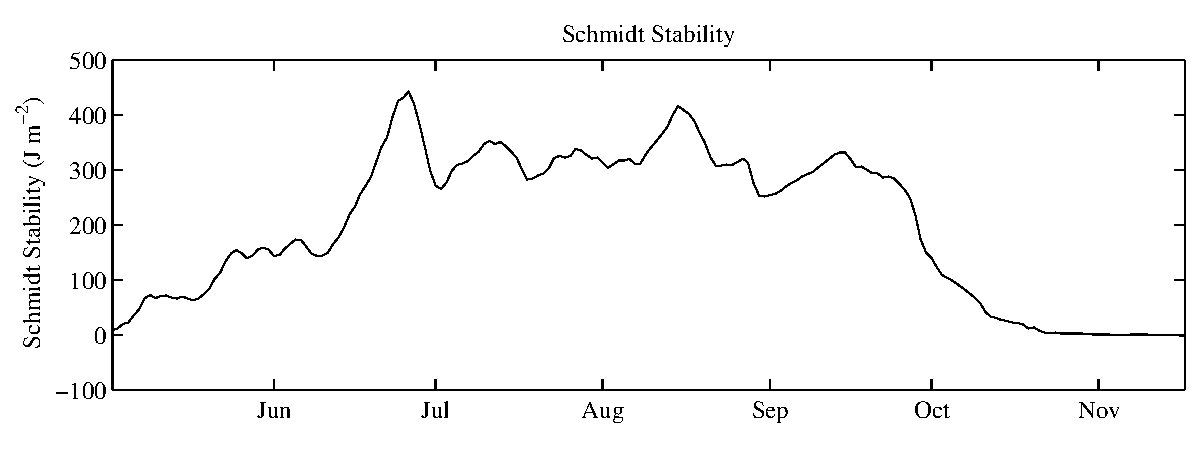
\includegraphics[width=.25\textwidth]{figures/Sparkling_St.pdf}}
    \subfigure{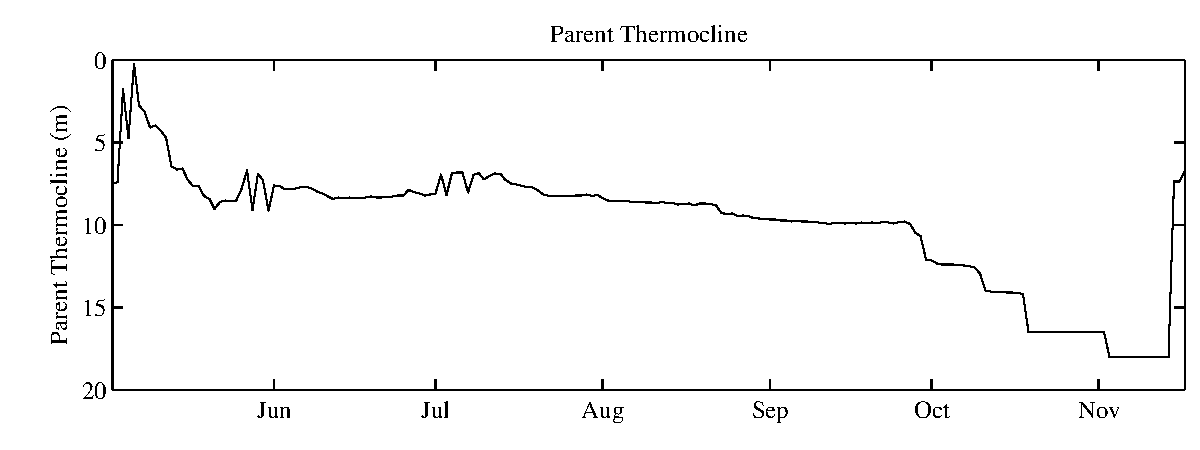
\includegraphics[width=.25\textwidth]{figures/Sparkling_SthermD.pdf}}\\
    \subfigure{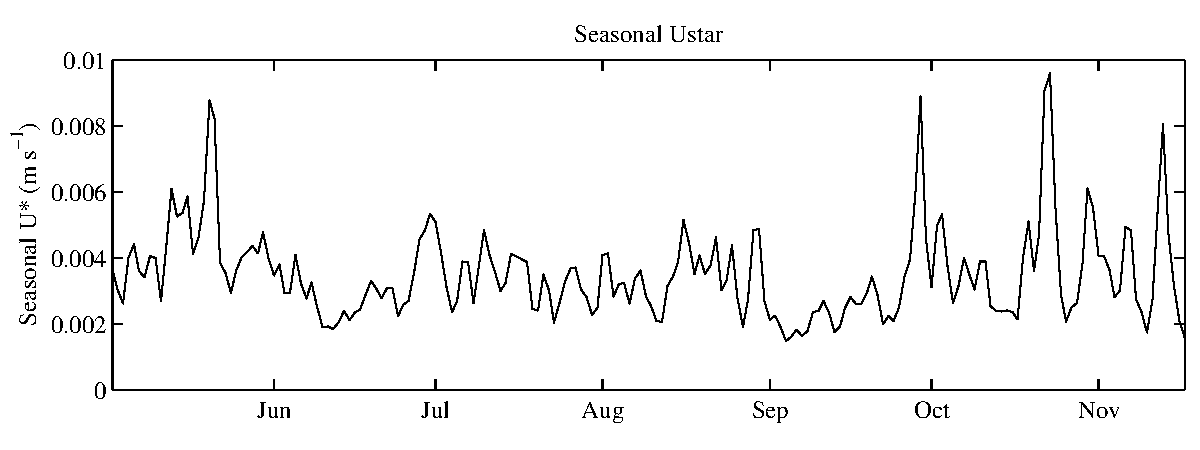
\includegraphics[width=.25\textwidth]{figures/Sparkling_SuSt.pdf}}
    \subfigure{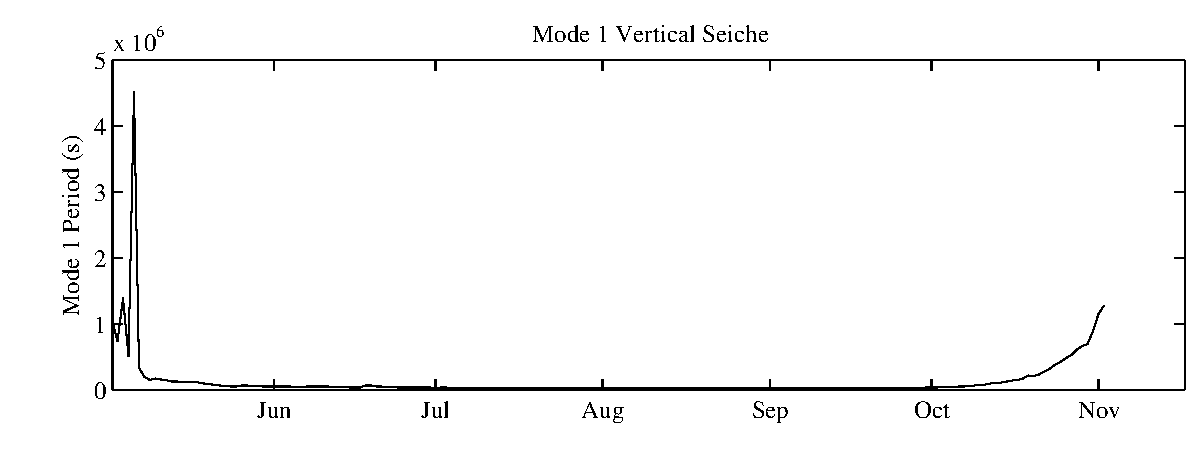
\includegraphics[width=.25\textwidth]{figures/Sparkling_T1.pdf}}
    \subfigure{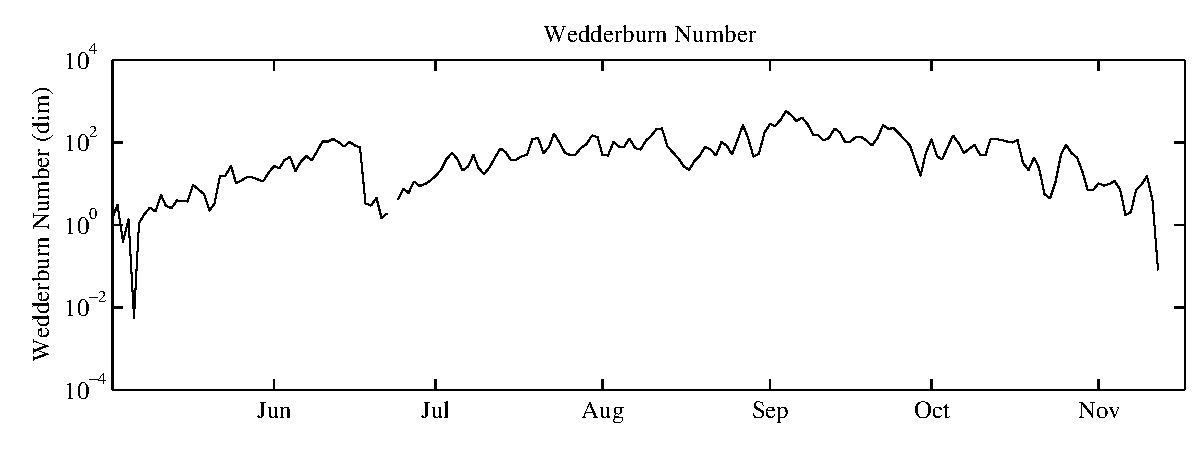
\includegraphics[width=.25\textwidth]{figures/Sparkling_W.pdf}}\\
    \subfigure{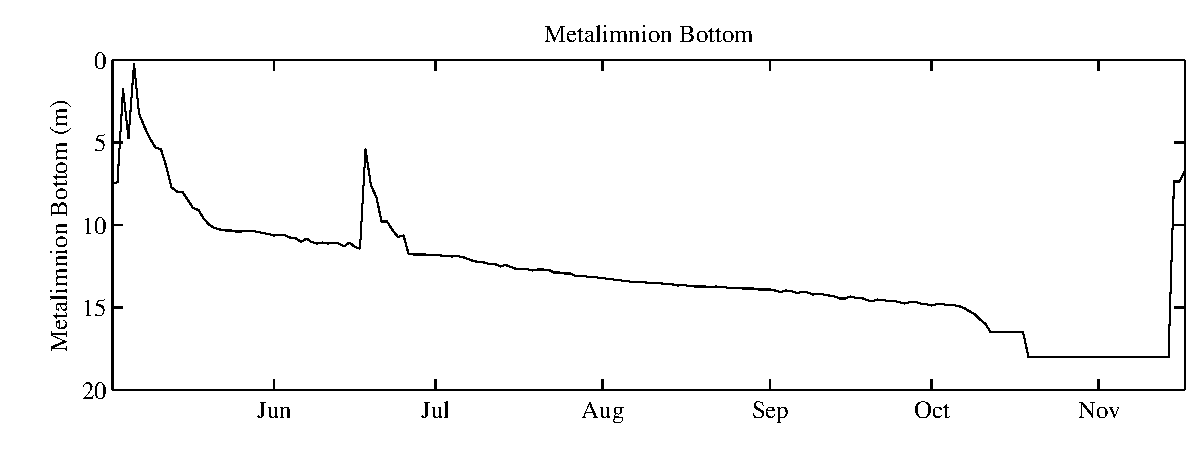
\includegraphics[width=.25\textwidth]{figures/Sparkling_metaB.pdf}}
    \subfigure{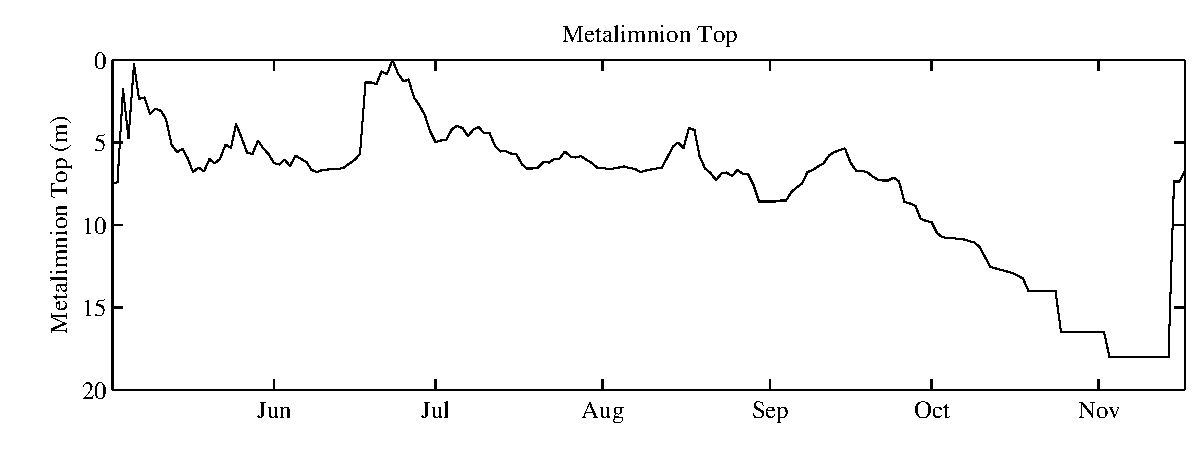
\includegraphics[width=.25\textwidth]{figures/Sparkling_metaT.pdf}}
    \subfigure{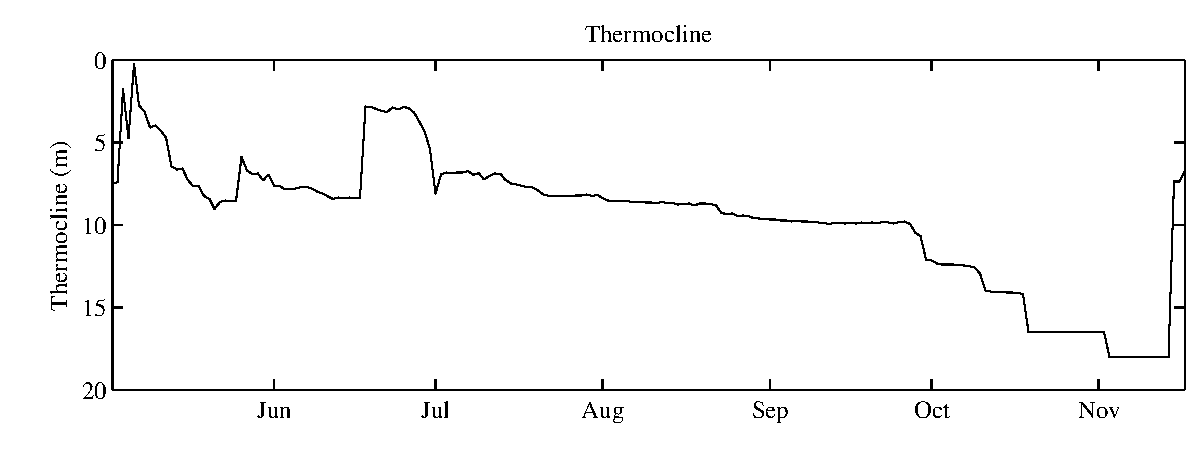
\includegraphics[width=.25\textwidth]{figures/Sparkling_thermD.pdf}}\\
    \subfigure{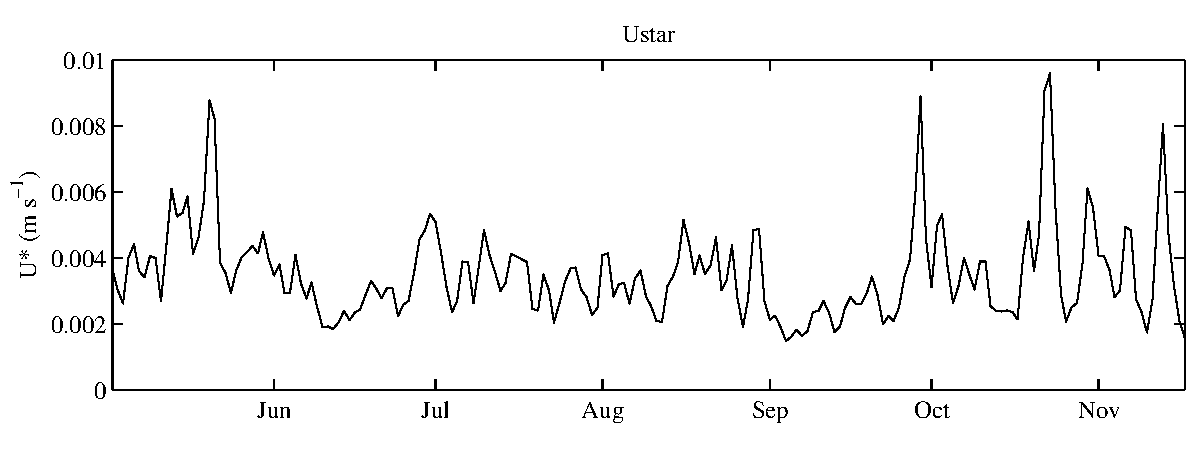
\includegraphics[width=.25\textwidth]{figures/Sparkling_uSt.pdf}}
    \subfigure{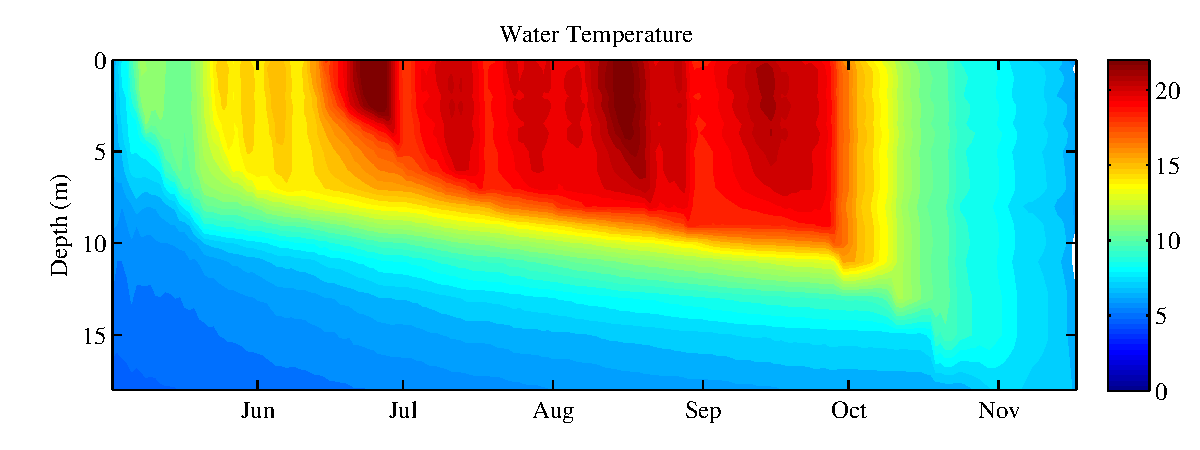
\includegraphics[width=.25\textwidth]{figures/Sparkling_wTemp.pdf}}
    \subfigure{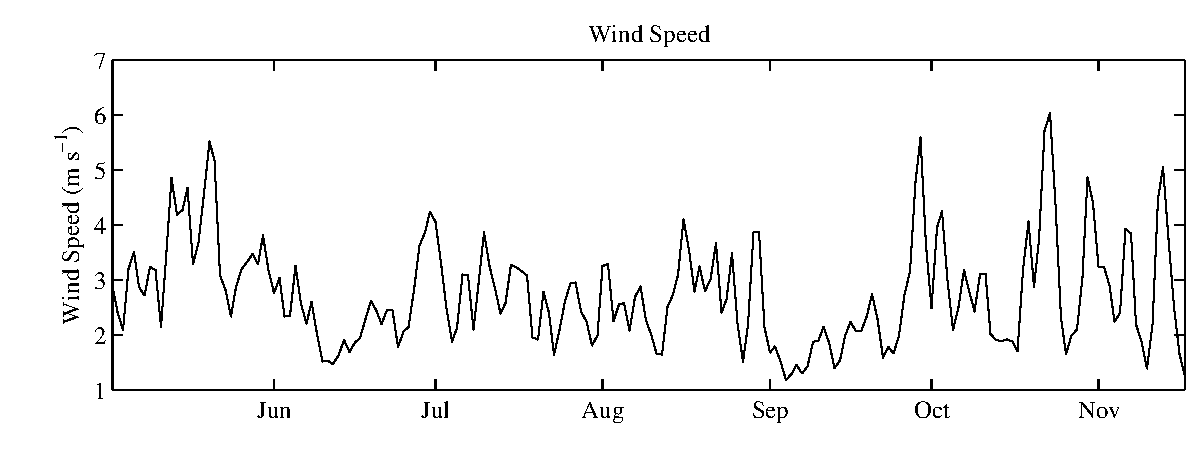
\includegraphics[width=.25\textwidth]{figures/Sparkling_wndSpd.pdf}}
  \end{figure}
\end{frame}

\titleframe{Matlab WPS}

\begin{frame}[t]{Matlab WPS}
  \begin{itemize}
    \item Offering Matlab functions as WPS processes
    \item Configuration with simple YAML file
  \end{itemize}
\end{frame}

\begin{frame}[fragile]{Matlab WPS --- Example}
  \begin{columns}
    \column{.39\textwidth}
    \lstinputlisting[language=Matlab]{listings/matlab-add-function.m}
    \pause
    \lstinputlisting{listings/matlab-add-process-configuration.yaml}
    \pause
    \column{.61\textwidth}
    \lstinputlisting[language=XML]{listings/matlab-add-process-description.xml}
  \end{columns}
\end{frame}

\begin{frame}[c,fragile]{Matlab WPS --- Websockets}
  \begin{columns}
    \column{.45\textwidth}
    \lstinputlisting{listings/websocket-handshake-request.txt}
    \pause
    \column{.45\textwidth}
    \lstinputlisting{listings/websocket-handshake-response.txt}
  \end{columns}
  \pause
  \begin{columns}
  \column{.45\textwidth}
  \column{.45\textwidth}
  Widely supported:
  \begin{itemize}
    \item IE \textgreater10
    \item Firefox \textgreater6
    \item Chrome \textgreater14
    \item Safari \textgreater6
    \item Opera \textgreater12.1
  \end{itemize}
  \end{columns}
\end{frame}

\begin{frame}[c,fragile]{Matlab WPS --- Accessing Matlab from the Web}
  \begin{columns}
    \column{.37\textwidth}
    \lstinputlisting[language=Matlab]{listings/matlab-add-function.m}
    \pause
    \lstinputlisting{listings/matlab-connector.sh}
    \pause
    \column{.63\textwidth}
    \lstinputlisting[language=JavaScript]{listings/matlab-add-javascript-client.js}
  \end{columns}
\end{frame}

\titleframe{Lake Analyzer WPS}

\begin{frame}[t]{Lake Analyzer WPS}
  \begin{itemize}
    \item simple implementation using the \emph{Matlab WPS}
    \item small modifications to the script to allow file transfers
    \item wrapper function to get rid of configuration files
  \end{itemize}
\end{frame}

\begin{frame}[c,fragile]{Lake Analyzer WPS --- Wrapper Function}
    \begin{center}
      \lstinputlisting[language=Matlab,lastline=10]{listings/lake-analyzer-wps-wrapper.m}
    \end{center}
\end{frame}

\begin{frame}[c,fragile]{Lake Analyzer WPS --- Configuration}
    \begin{center}
      \lstinputlisting[lastline=40]{listings/lake-analyzer-wps-configuration.yaml}
    \end{center}
\end{frame}

\begin{frame}[c,fragile]{Lake Analyzer WPS --- Process Description}
    \begin{center}
      \lstinputlisting[language=XML,lastline=40]{listings/lake-analyzer-wps-process-description.xml}
    \end{center}
\end{frame}

\begin{frame}[c,fragile]{Lake Analyzer WPS --- Process Description}
    \begin{center}
      \lstinputlisting[language=XML,firstline=451,lastline=484]{listings/lake-analyzer-wps-process-description.xml}
    \end{center}
\end{frame}

\begin{frame}[c,fragile]{Lake Analyzer WPS --- Example Request}
    \begin{center}
      \lstinputlisting[language=XML,lastline=40]{listings/lake-analyzer-wps-request.xml}
    \end{center}
\end{frame}

\begin{frame}[c,fragile]{Lake Analyzer WPS --- Example Response}
    \begin{center}
      \lstinputlisting[language=XML,lastline=20]{listings/lake-analyzer-wps-response.xml}
    \end{center}
\end{frame}

\begin{frame}[c,fragile]{Lake Analyzer WPS --- Example Response}
    \begin{center}
      \lstinputlisting[language=XML,firstline=426,lastline=490]{listings/lake-analyzer-wps-response.xml}
    \end{center}
\end{frame}

\begin{frame}[c,fragile]{Lake Analyzer WPS --- Example Response}
  \begin{figure}
    \centering
    \subfigure{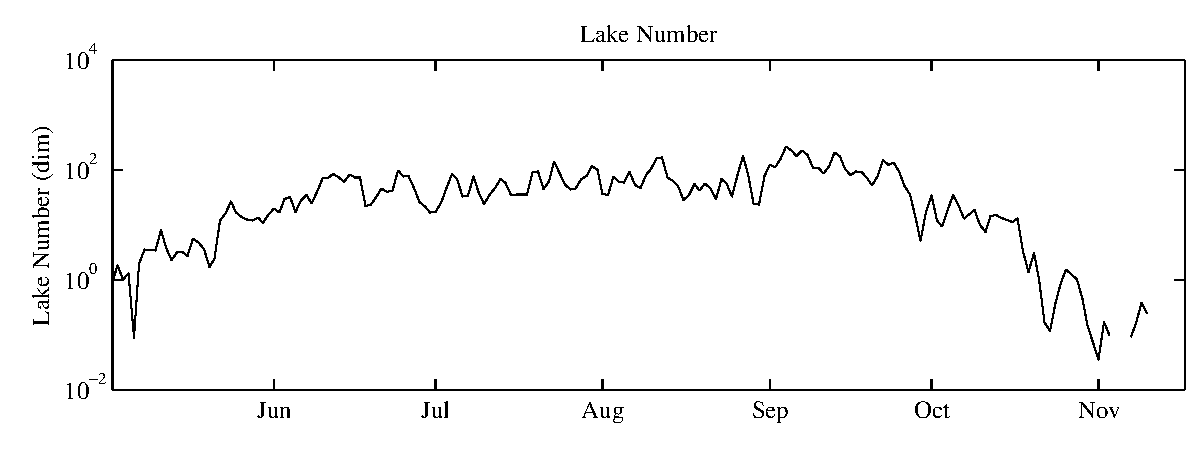
\includegraphics[width=.25\textwidth]{figures/Sparkling_Ln.pdf}}
    \subfigure{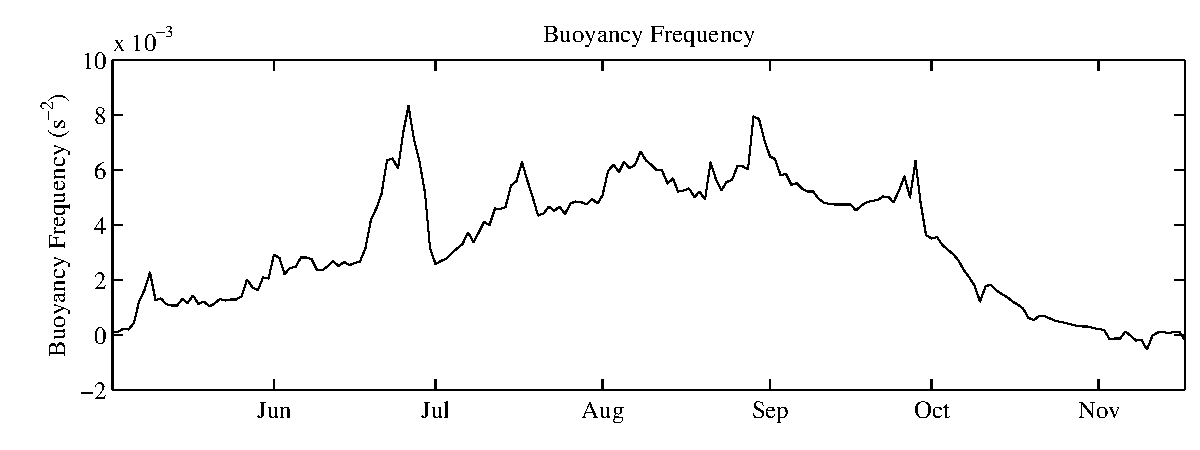
\includegraphics[width=.25\textwidth]{figures/Sparkling_N2.pdf}}
    \subfigure{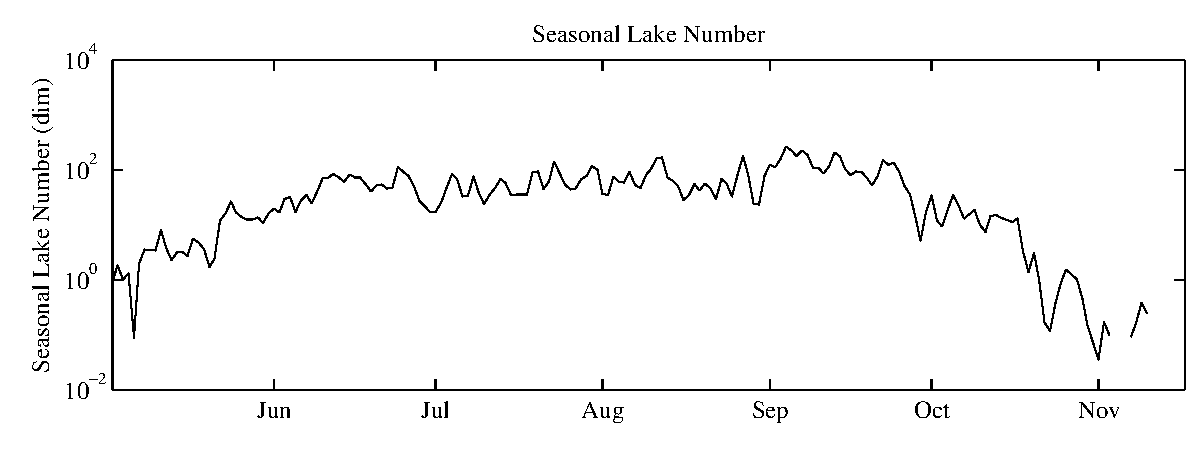
\includegraphics[width=.25\textwidth]{figures/Sparkling_SLn.pdf}}\\
    \subfigure{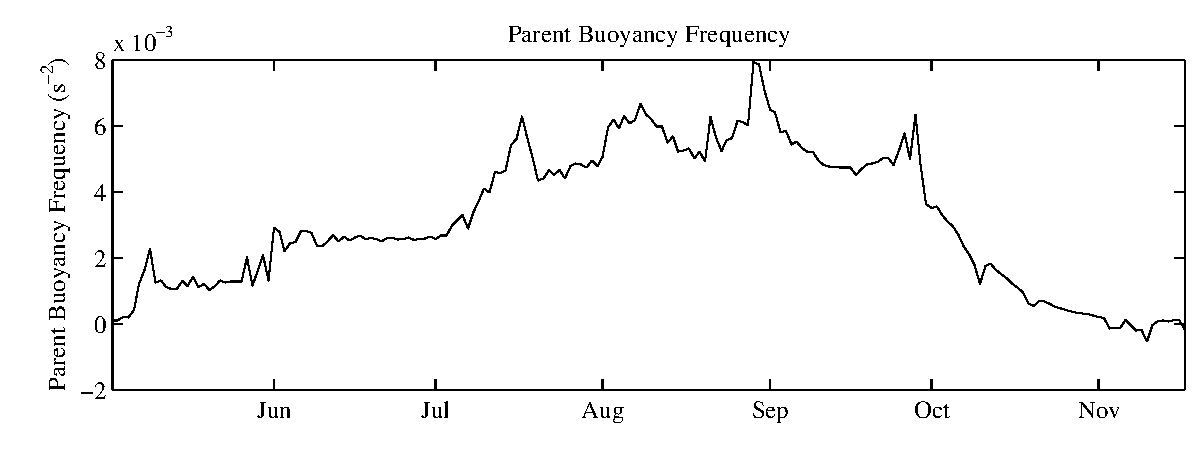
\includegraphics[width=.25\textwidth]{figures/Sparkling_SN2.pdf}}
    \subfigure{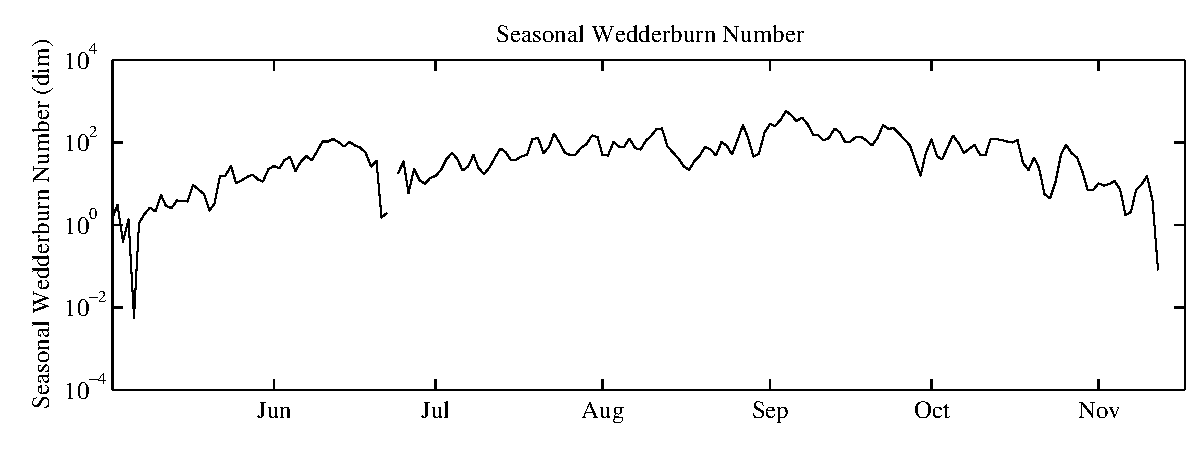
\includegraphics[width=.25\textwidth]{figures/Sparkling_SW.pdf}}
    \subfigure{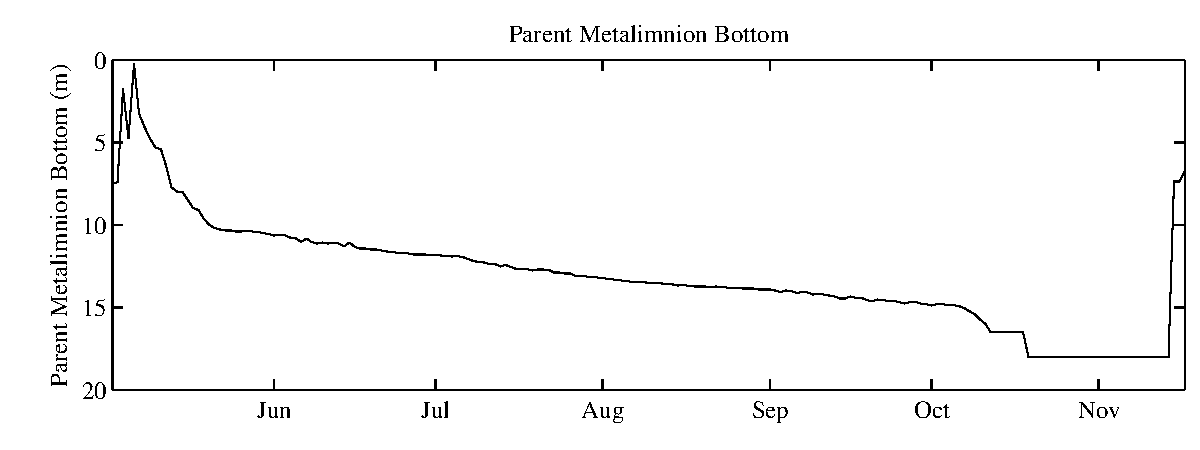
\includegraphics[width=.25\textwidth]{figures/Sparkling_SmetaB.pdf}}\\
    \subfigure{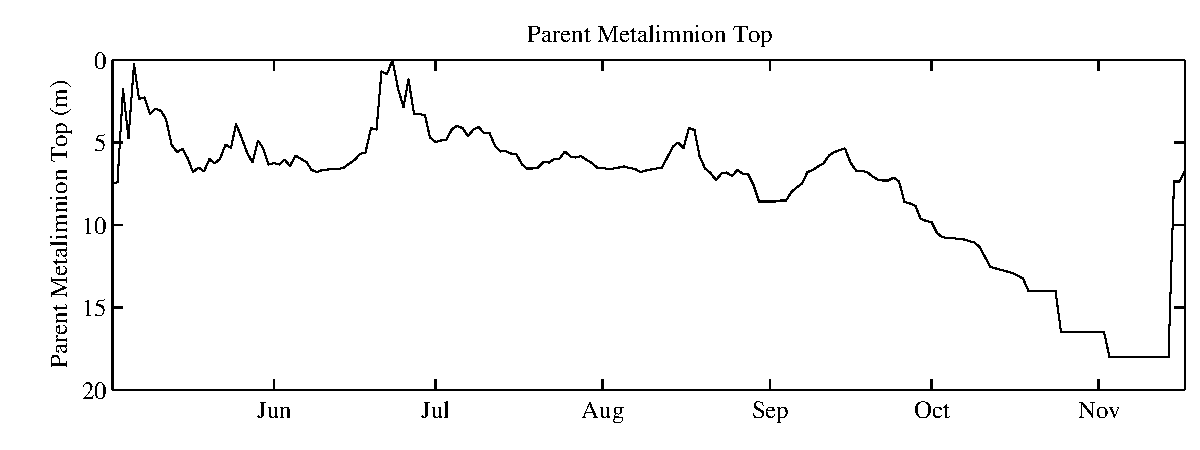
\includegraphics[width=.25\textwidth]{figures/Sparkling_SmetaT.pdf}}
    \subfigure{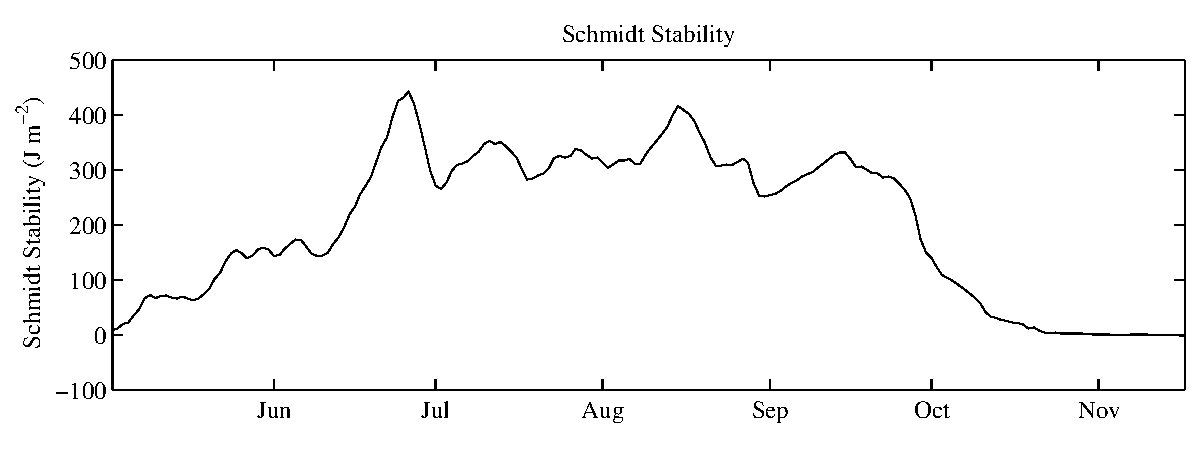
\includegraphics[width=.25\textwidth]{figures/Sparkling_St.pdf}}
    \subfigure{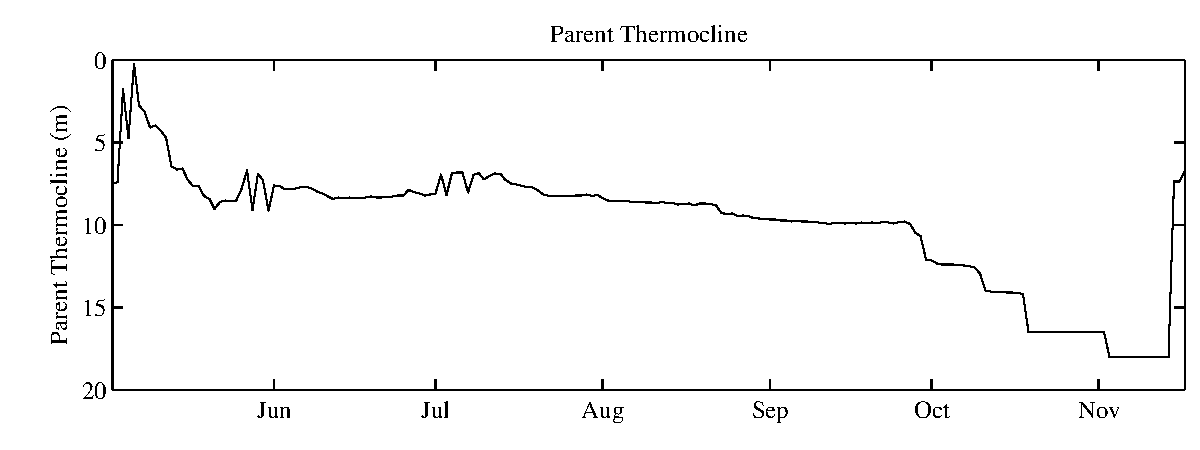
\includegraphics[width=.25\textwidth]{figures/Sparkling_SthermD.pdf}}\\
    \subfigure{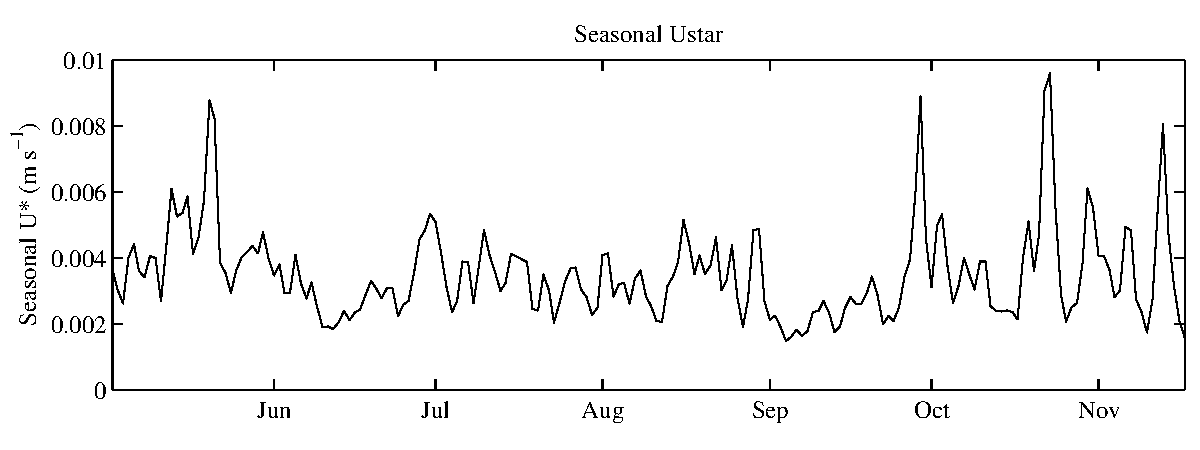
\includegraphics[width=.25\textwidth]{figures/Sparkling_SuSt.pdf}}
    \subfigure{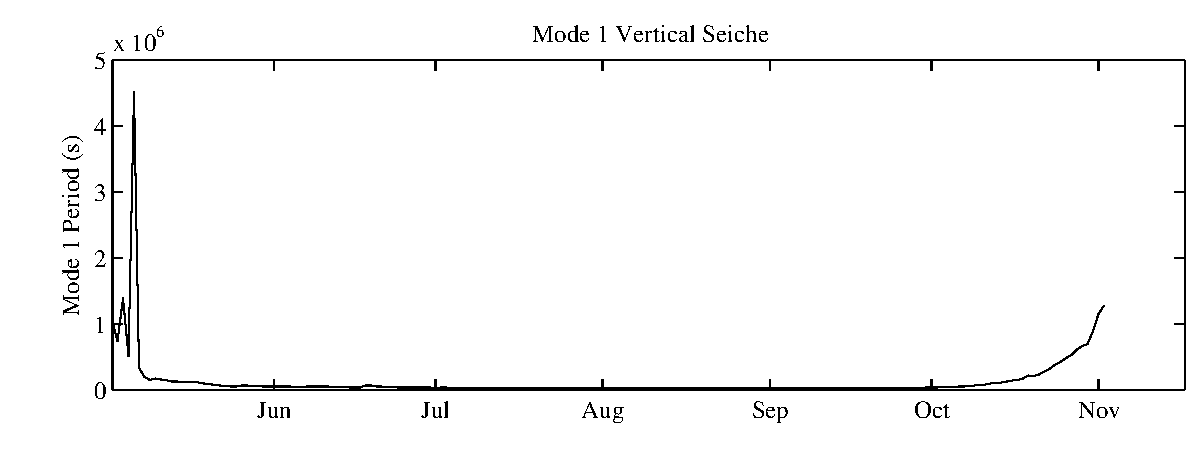
\includegraphics[width=.25\textwidth]{figures/Sparkling_T1.pdf}}
    \subfigure{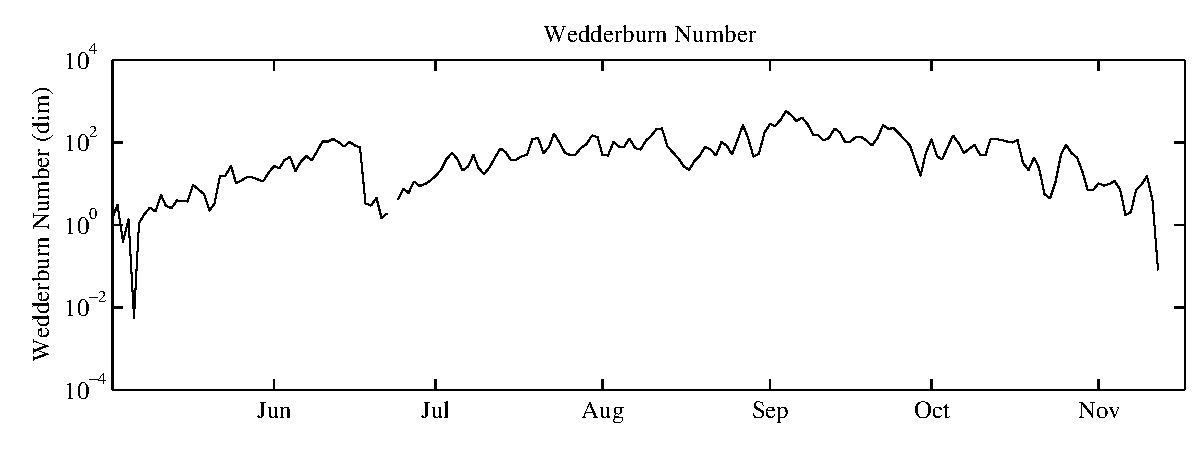
\includegraphics[width=.25\textwidth]{figures/Sparkling_W.pdf}}\\
    \subfigure{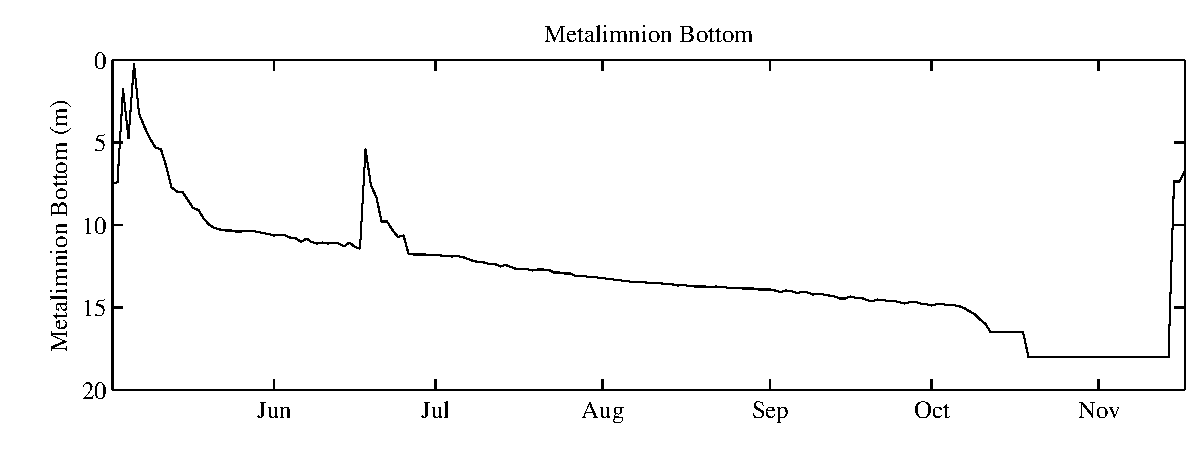
\includegraphics[width=.25\textwidth]{figures/Sparkling_metaB.pdf}}
    \subfigure{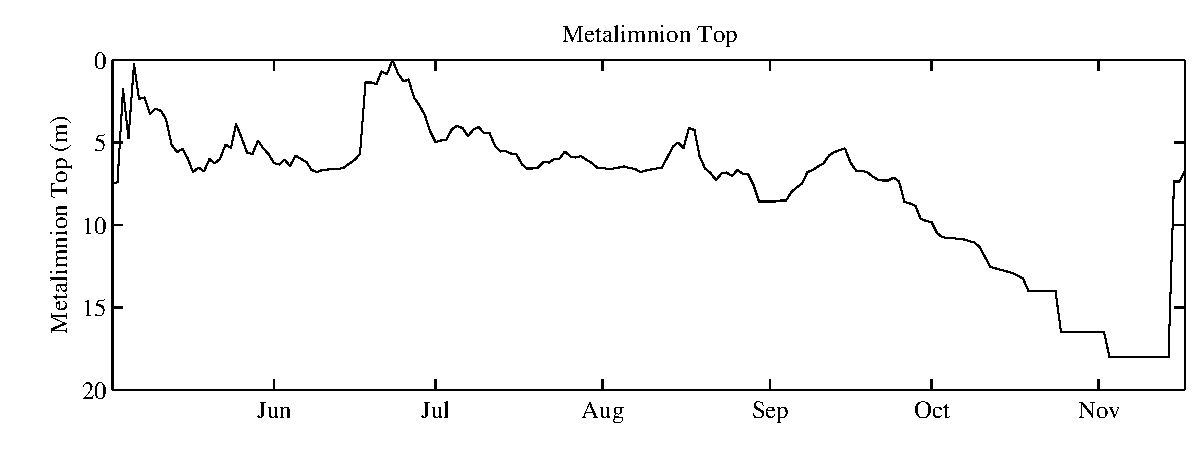
\includegraphics[width=.25\textwidth]{figures/Sparkling_metaT.pdf}}
    \subfigure{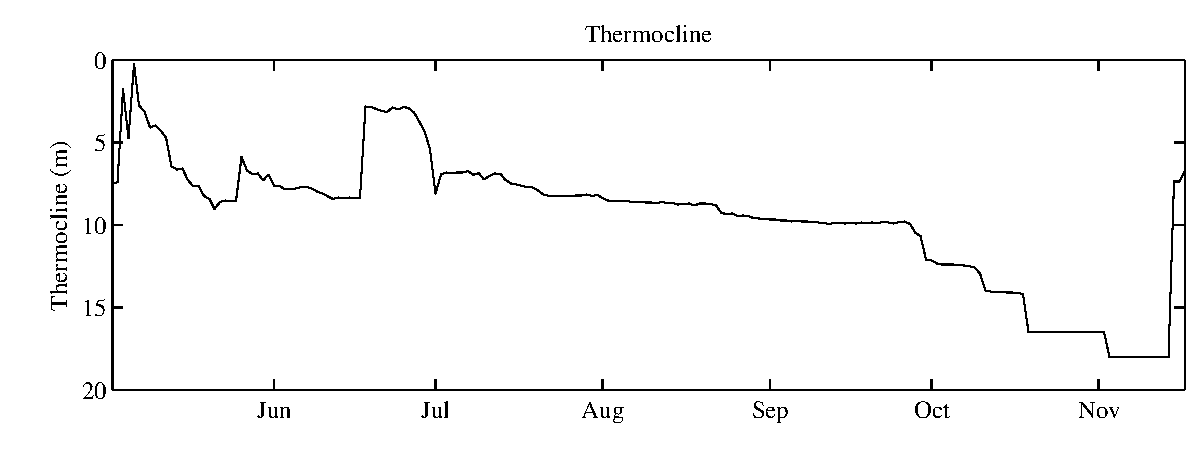
\includegraphics[width=.25\textwidth]{figures/Sparkling_thermD.pdf}}\\
    \subfigure{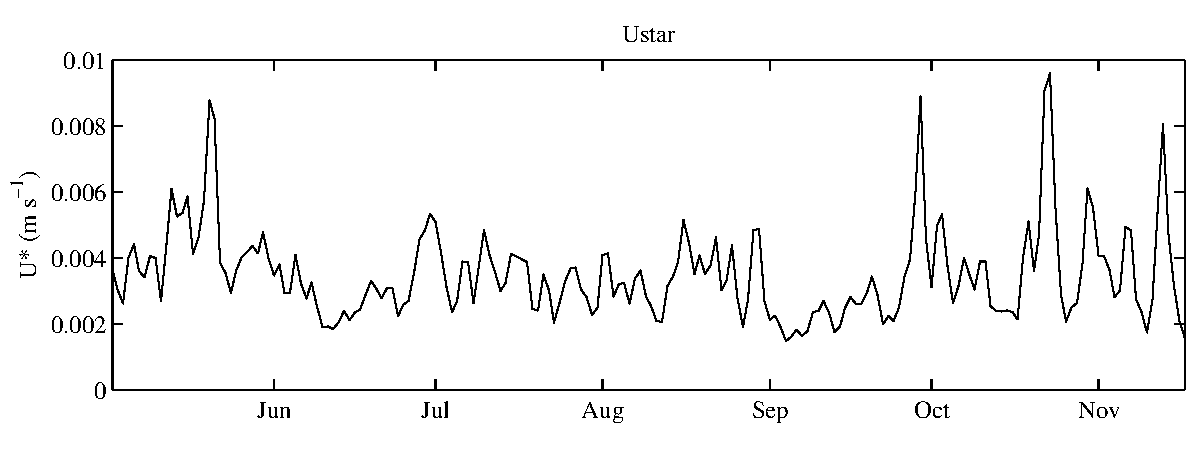
\includegraphics[width=.25\textwidth]{figures/Sparkling_uSt.pdf}}
    \subfigure{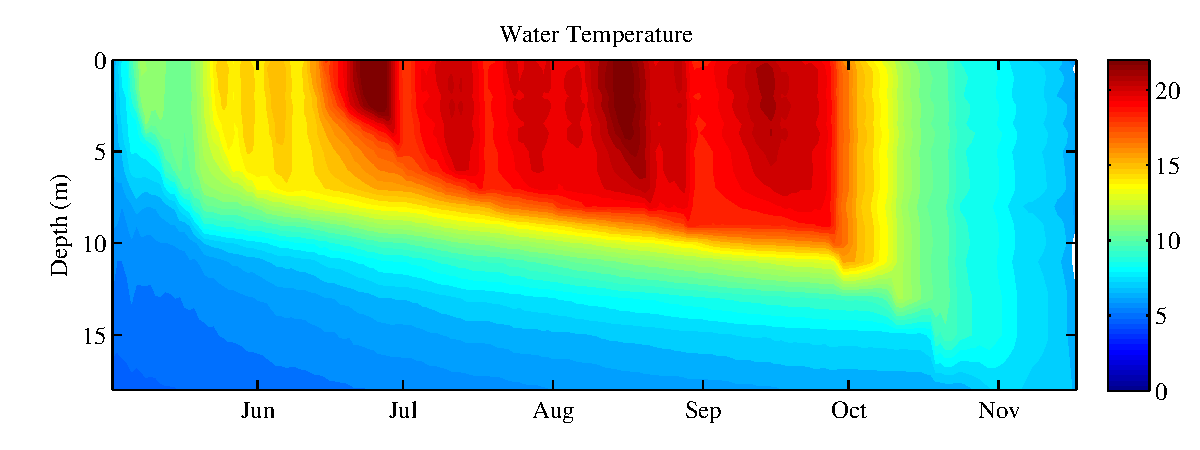
\includegraphics[width=.25\textwidth]{figures/Sparkling_wTemp.pdf}}
    \subfigure{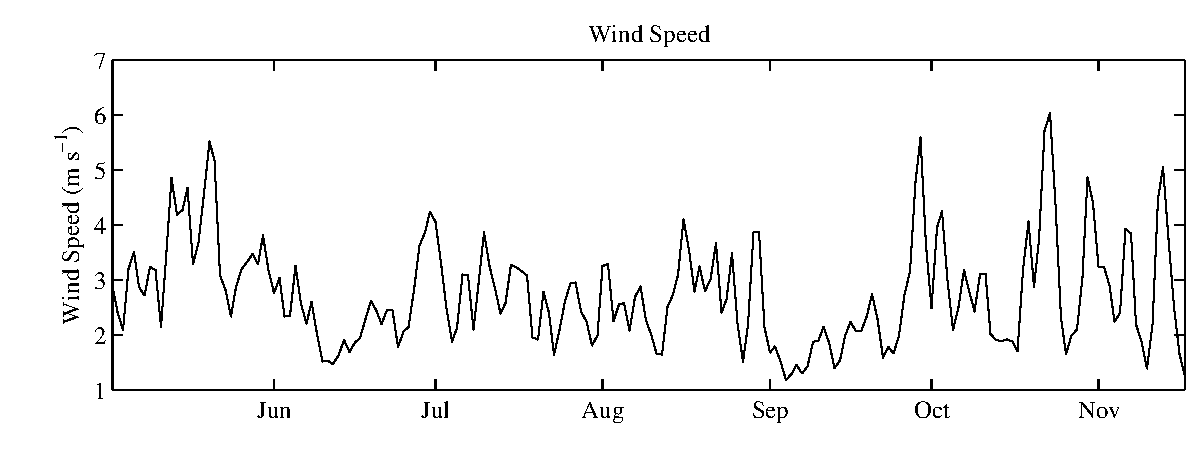
\includegraphics[width=.25\textwidth]{figures/Sparkling_wndSpd.pdf}}
  \end{figure}
\end{frame}

\titleframe{Streaming WPS}

\begin{frame}[t]{Streaming WPS}
  \begin{itemize}
    \item
  \end{itemize}
\end{frame}

\begin{frame}[c,fragile]{Streaming WPS --- Sequence Diagram}
  \begin{figure}
    \begin{center}
      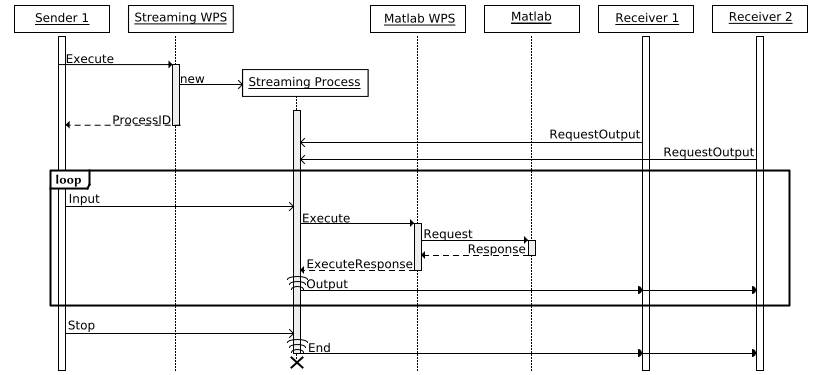
\includegraphics[width=\textwidth]{figures/sequence-diagram.pdf}
    \end{center}
  \end{figure}
\end{frame}

\begin{frame}[c,fragile]{Streaming WPS --- Sequence Diagram}
  \begin{figure}
    \begin{center}
      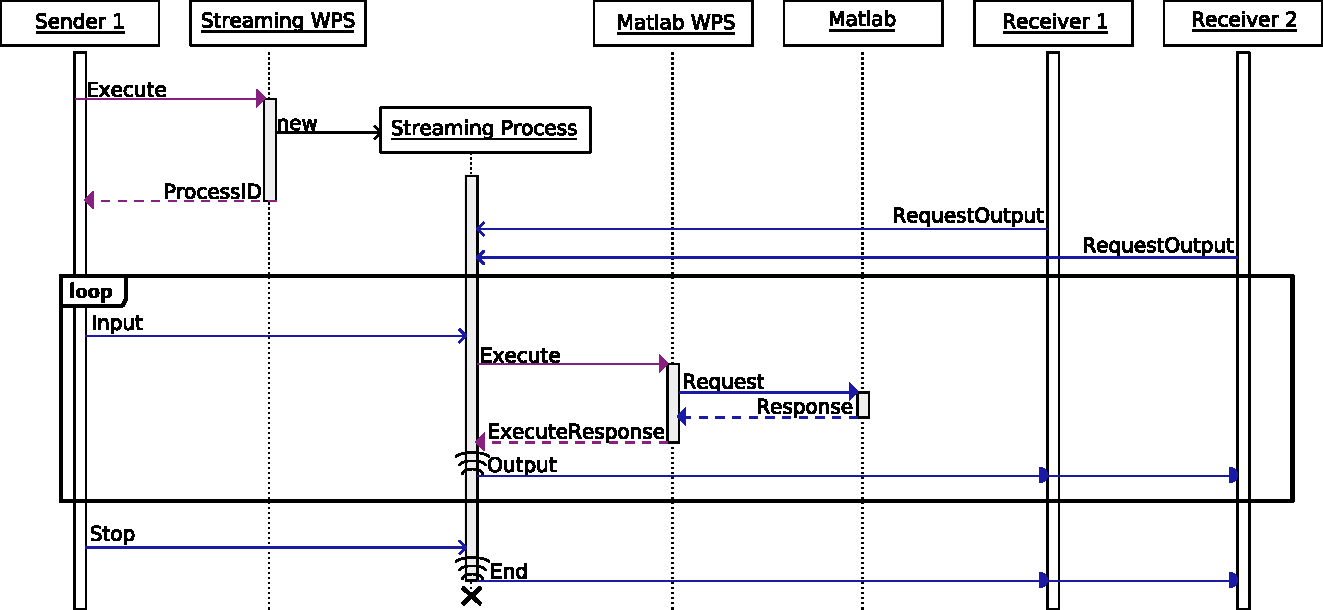
\includegraphics[width=\textwidth]{figures/sequence-diagram2.pdf}
    \end{center}
  \end{figure}
\end{frame}

\begin{frame}{Streaming WPS --- Input Types}
  \begin{itemize}
    \item Streaming Inputs
    \pause
    \begin{itemize}
      \item submitted with \texttag{stream}{InputMessage}
      \item of type \texttag{wps}{Input}
    \end{itemize}
    \pause
    \item Static Inputs
    \pause
    \begin{itemize}
      \item submitted with initial \texttag{wps}{Execute}
      \item merged with inputs of every streaming iteration
      \item of type \texttag{wps}{Input}
    \end{itemize}
    \pause
    \item Reference Inputs
    \pause
    \begin{itemize}
      \item submitted with \texttag{stream}{InputMessage}
      \item references the output of a previous or upcoming streaming iteration
    \end{itemize}
    \pause
    \item Polling Inputs
  \end{itemize}
\end{frame}

\begin{frame}[c,fragile]{Streaming WPS --- Input Message}
    \begin{center}
      \lstinputlisting[language=XML]{listings/streaming-input-message.xml}
    \end{center}
\end{frame}

\begin{frame}[c,fragile]{Streaming WPS --- Ouput Request Message}
    \begin{center}
      \lstinputlisting[language=XML]{listings/streaming-output-request-message.xml}
    \end{center}
\end{frame}

\begin{frame}[c,fragile]{Streaming WPS --- Output Message}
    \begin{center}
      \lstinputlisting[language=XML]{listings/streaming-output-message.xml}
    \end{center}
\end{frame}

\begin{frame}[c,fragile]{Streaming WPS --- Stop Message}
    \begin{center}
      \lstinputlisting[language=XML]{listings/streaming-stop-message.xml}
    \end{center}
\end{frame}

\begin{frame}[t]{Streaming WPS --- Handling Dependencies}
  \begin{itemize}
    \item Clients declare dependencies to other streaming iterations (or their outputs)
    \item Automatic declaration of (spatial) dependencies not possibe as it is use case and format specific
    \item Process waits for all dependencies to become available
    \item Checking for cyclic dependencies using a directed acyclic graph and topological sorting (BFS)
  \end{itemize}
\end{frame}

\titleframe{Current Status}

\begin{frame}[t]{Current Status}
  \begin{itemize}
    \done Matlab WPS
    \done Lake Analyzer WPS
    \missing Streaming WPS
    \begin{itemize}
      \done Implementation
      \missing Testing \& Bug Fixing
    \end{itemize}
    \missing Webapp showcasing the process chain
  \end{itemize}
  \begin{itemize}
    \item \url{https://github.com/autermann/matlab-connector}
    \item \url{https://github.com/autermann/matlab-wps}
    \item \url{https://github.com/autermann/Lake-Analyzer}
    \item \url{https://github.com/autermann/streaming-wps}
  \end{itemize}
\end{frame}

\begin{frame}
  \vfill
  \begin{center}
    \emph{Thanks. Questions?}
  \end{center}
  \vfill
\end{frame}

\end{document}
